\documentclass[12pt]{article}
\usepackage{amsfonts, amssymb, amsmath, amsthm}
\usepackage[margin=1in]{geometry}
\usepackage{tikz}
\usetikzlibrary{patterns, decorations.pathreplacing}

\pagestyle{myheadings}
\markright{Explainer: Rudin 2.6 — Limit Points and Closure\hfill}

\newcommand{\R}{\mathbb{R}}

\begin{document}

\begin{center}
    \textbf{\Large Understanding Limit Points and Closure}\\[0.5em]
    \large A visual guide to Rudin 2.6
\end{center}

\section{What is a Limit Point?}

A point $p$ is a \textbf{limit point} of a set $E$ if every neighborhood of $p$ contains at least one point of $E$ \emph{different from $p$}.

\begin{center}
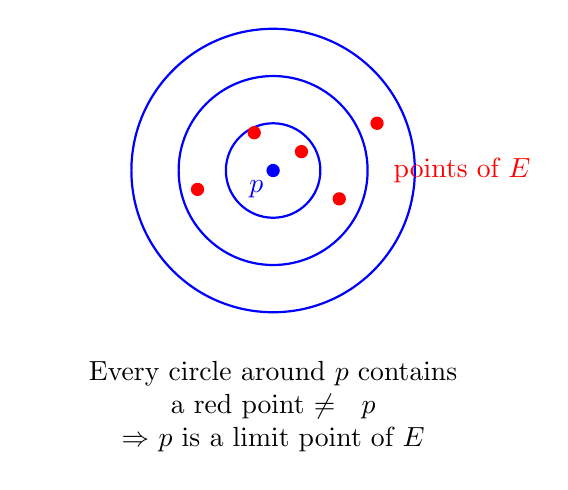
\begin{tikzpicture}[scale=1.2]
    % Draw the point p
    \fill[blue] (0,0) circle (2pt) node[below left] {$p$};

    % Draw neighborhoods
    \draw[blue, thick] (0,0) circle (1.5);
    \draw[blue, thick] (0,0) circle (1.0);
    \draw[blue, thick] (0,0) circle (0.5);

    % Draw points of E
    \fill[red] (0.3, 0.2) circle (2pt);
    \fill[red] (0.7, -0.3) circle (2pt);
    \fill[red] (1.1, 0.5) circle (2pt);
    \fill[red] (-0.2, 0.4) circle (2pt);
    \fill[red] (-0.8, -0.2) circle (2pt);

    \node[red] at (2, 0) {points of $E$};

    \node[text width=6cm, align=center] at (0, -2.5) {Every circle around $p$ contains\\a red point $\neq p$\\$\Rightarrow$ $p$ is a limit point of $E$};
\end{tikzpicture}
\end{center}

\subsection{Limit Point vs Element of the Set}

\textbf{Important:} A limit point doesn't have to be \emph{in} the set!

\begin{center}
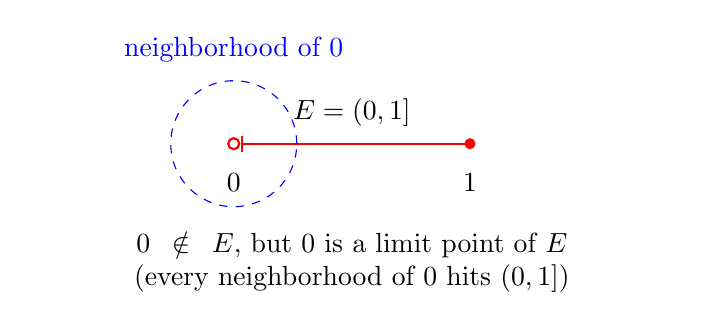
\begin{tikzpicture}[scale=1]
    % Example: E = (0,1), limit point at 0
    \draw[thick, red] (0.1, 0) -- (3, 0);
    \draw[red, thick] (0.1, 0.1) -- (0.1, -0.1);
    \draw[red, thick, fill=white] (0, 0) circle (2pt);
    \fill[red] (3, 0) circle (2pt);

    \node at (1.5, 0.4) {$E = (0, 1]$};
    \node at (0, -0.5) {$0$};
    \node at (3, -0.5) {$1$};

    \draw[blue, dashed] (0, 0) circle (0.8);
    \node[blue] at (0, 1.2) {neighborhood of $0$};

    \node[text width=8cm, align=center] at (1.5, -1.5) {$0 \notin E$, but $0$ is a limit point of $E$\\(every neighborhood of $0$ hits $(0,1]$)};
\end{tikzpicture}
\end{center}

\section{The Set of Limit Points: $E'$}

We write $E'$ for the set of \emph{all} limit points of $E$.

\begin{center}
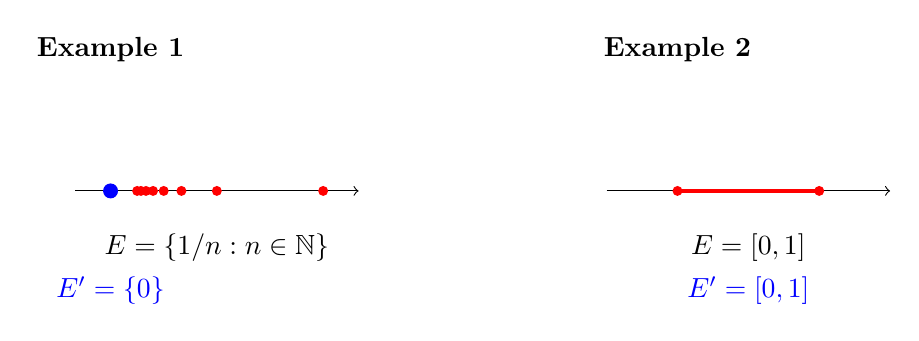
\begin{tikzpicture}[scale=0.9]
    % Example 1: E = {1/n}
    \begin{scope}[xshift=-4.5cm]
        \node at (0, 2) {\textbf{Example 1}};
        \draw[->] (-0.5, 0) -- (3.5, 0);

        % Points 1/n
        \foreach \n in {1,2,3,4,5,6,7,8} {
            \pgfmathsetmacro{\x}{3/\n}
            \fill[red] (\x, 0) circle (2pt);
        }
        \fill[blue] (0, 0) circle (3pt);

        \node at (1.5, -0.8) {$E = \{1/n : n \in \mathbb{N}\}$};
        \node[blue] at (0, -1.4) {$E' = \{0\}$};
    \end{scope}

    % Example 2: E = [0,1]
    \begin{scope}[xshift=3.5cm]
        \node at (0, 2) {\textbf{Example 2}};
        \draw[->] (-1, 0) -- (3, 0);

        \draw[red, very thick] (0, 0) -- (2, 0);
        \fill[red] (0, 0) circle (2pt);
        \fill[red] (2, 0) circle (2pt);

        \node at (1, -0.8) {$E = [0, 1]$};
        \node[blue] at (1, -1.4) {$E' = [0, 1]$};
    \end{scope}
\end{tikzpicture}
\end{center}

\section{What Does ``$E'$ is Closed'' Mean?}

A set is \textbf{closed} if it contains all its limit points.

So ``$E'$ is closed'' means: $(E')' \subseteq E'$

\begin{center}
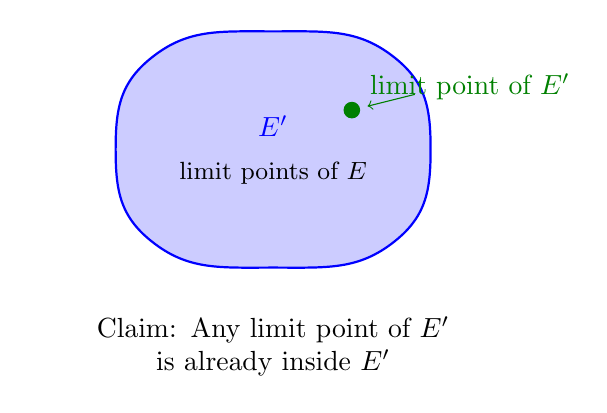
\begin{tikzpicture}[scale=1]
    % Visual representation
    \draw[thick, blue, fill=blue!20] plot[smooth cycle, tension=0.8] coordinates {(-2,0) (-1.5,1.2) (0,1.5) (1.5,1.2) (2,0) (1.5,-1.2) (0,-1.5) (-1.5,-1.2)};

    \node[blue] at (0, 0.3) {$E'$};
    \node at (0, -0.3) {\small limit points of $E$};

    % Show a limit point of E'
    \fill[green!50!black] (1, 0.5) circle (3pt);
    \node[green!50!black] at (2.5, 0.8) {limit point of $E'$};
    \draw[->, green!50!black] (1.8, 0.7) -- (1.2, 0.55);

    \node[text width=6cm, align=center] at (0, -2.5) {Claim: Any limit point of $E'$\\is already inside $E'$};
\end{tikzpicture}
\end{center}

\section{The Proof Strategy}

To show $E'$ is closed, we show $(E')' \subseteq E'$.

\textbf{Setup:} Let $p \in (E')'$ (a limit point of $E'$). We must show $p \in E'$.

\begin{center}
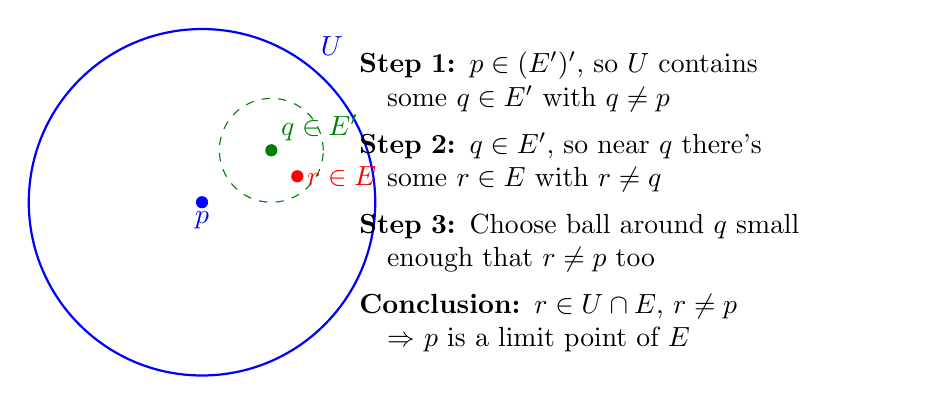
\begin{tikzpicture}[scale=1.1]
    % p and its neighborhood
    \fill[blue] (0,0) circle (2pt) node[below] {$p$};
    \draw[blue, thick] (0,0) circle (2);
    \node[blue] at (1.5, 1.8) {$U$};

    % q in E'
    \fill[green!50!black] (0.8, 0.6) circle (2pt) node[above right] {$q \in E'$};

    % Small ball around q
    \draw[green!50!black, dashed] (0.8, 0.6) circle (0.6);

    % r in E
    \fill[red] (1.1, 0.3) circle (2pt) node[right] {$r \in E$};

    \node[text width=7cm, align=left] at (5, 0) {
        \textbf{Step 1:} $p \in (E')'$, so $U$ contains\\
        \hspace{1em}some $q \in E'$ with $q \neq p$\\[0.5em]
        \textbf{Step 2:} $q \in E'$, so near $q$ there's\\
        \hspace{1em}some $r \in E$ with $r \neq q$\\[0.5em]
        \textbf{Step 3:} Choose ball around $q$ small\\
        \hspace{1em}enough that $r \neq p$ too\\[0.5em]
        \textbf{Conclusion:} $r \in U \cap E$, $r \neq p$\\
        \hspace{1em}$\Rightarrow$ $p$ is a limit point of $E$
    };
\end{tikzpicture}
\end{center}

\section{The Key Trick: Excluding $p$}

Why do we need $r \neq p$? Because the definition of limit point requires a point \emph{different from $p$}.

\begin{center}
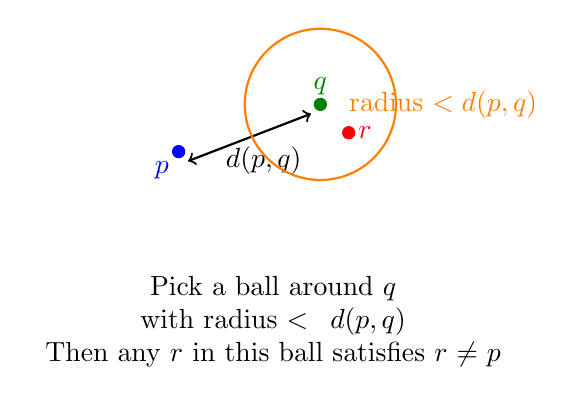
\begin{tikzpicture}[scale=1.2]
    \fill[blue] (0,0) circle (2pt) node[below left] {$p$};
    \fill[green!50!black] (1.5, 0.5) circle (2pt) node[above] {$q$};

    % Distance
    \draw[<->, thick] (0.1, -0.1) -- (1.4, 0.4);
    \node at (0.9, -0.1) {$d(p,q)$};

    % Ball around q that excludes p
    \draw[orange, thick] (1.5, 0.5) circle (0.8);
    \node[orange] at (2.8, 0.5) {radius $< d(p,q)$};

    \fill[red] (1.8, 0.2) circle (2pt) node[right] {$r$};

    \node[text width=6cm, align=center] at (1, -1.8) {Pick a ball around $q$ with radius $< d(p,q)$\\Then any $r$ in this ball satisfies $r \neq p$};
\end{tikzpicture}
\end{center}

\section{Part 2: $E$ and $\bar{E}$ Have the Same Limit Points}

Recall: $\bar{E} = E \cup E'$ (closure = set $\cup$ limit points)

\textbf{Claim:} $E' = (\bar{E})'$

\begin{center}
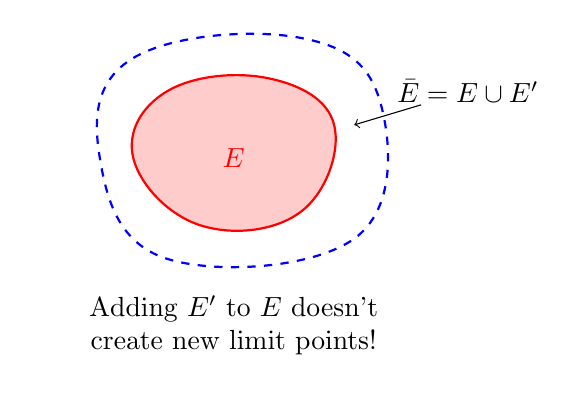
\begin{tikzpicture}[scale=0.85]
    % E
    \draw[red, thick, fill=red!20] plot[smooth cycle, tension=0.7] coordinates {(-1.5,0) (-1,1) (0.5,1.2) (1.5,0.5) (1,-0.8) (-0.5,-1)};
    \node[red] at (0, 0) {$E$};

    % E' extending E
    \draw[blue, thick, dashed] plot[smooth cycle, tension=0.7] coordinates {(-2,0) (-1.5,1.5) (1,1.8) (2.2,0.8) (1.8,-1.2) (-1,-1.5)};

    \node at (3.5, 1) {$\bar{E} = E \cup E'$};
    \draw[->] (2.8, 0.8) -- (1.8, 0.5);

    \node[text width=5cm, align=center] at (0, -2.5) {Adding $E'$ to $E$ doesn't\\create new limit points!};
\end{tikzpicture}
\end{center}

\textbf{Why?}
\begin{itemize}
    \item $E \subseteq \bar{E}$, so limit points of $E$ are limit points of $\bar{E}$: $E' \subseteq (\bar{E})'$
    \item If $p$ is a limit point of $\bar{E}$, nearby points are in $E$ or $E'$. Either way, we can find points of $E$ nearby (using the Part 1 trick), so $p \in E'$: $(\bar{E})' \subseteq E'$
\end{itemize}

\section{Part 3: Do $E$ and $E'$ Have the Same Limit Points?}

\textbf{No!} Counterexample: $E = \{1/n : n \in \mathbb{N}\}$

\begin{center}
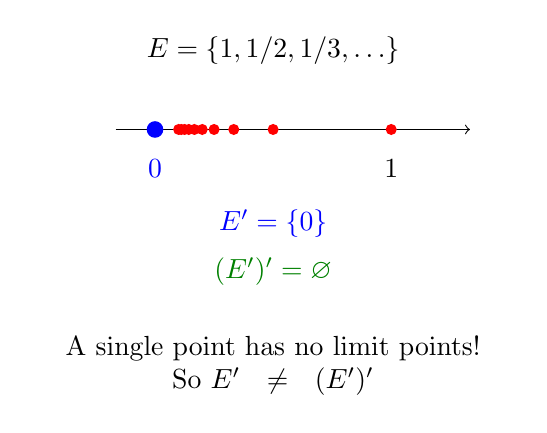
\begin{tikzpicture}[scale=1]
    \draw[->] (-0.5, 0) -- (4, 0);

    % Points 1/n
    \foreach \n in {1,2,3,4,5,6,7,8,9,10} {
        \pgfmathsetmacro{\x}{3/\n}
        \fill[red] (\x, 0) circle (2pt);
    }

    \fill[blue] (0, 0) circle (3pt);
    \node[blue] at (0, -0.5) {$0$};
    \node at (3, -0.5) {$1$};

    \node at (1.5, 1) {$E = \{1, 1/2, 1/3, \ldots\}$};
    \node[blue] at (1.5, -1.2) {$E' = \{0\}$};
    \node[green!50!black] at (1.5, -1.8) {$(E')' = \varnothing$};

    \node[text width=6cm, align=center] at (1.5, -3) {A single point has no limit points!\\So $E' \neq (E')'$};
\end{tikzpicture}
\end{center}

\end{document}
